\documentclass[12pt, titlepage]{article}

\usepackage{booktabs}
\usepackage{tabularx}
\usepackage{graphicx}
\graphicspath{{./images/}}
\usepackage{caption}
\usepackage{float}
\usepackage{hyperref}
\usepackage{pdflscape}
\hypersetup{
    colorlinks,
    citecolor=black,
    filecolor=black,
    linkcolor=red,
    urlcolor=blue
}
\usepackage[round]{natbib}

%% Comments
\usepackage{color}
\newif\ifcomments\commentstrue %displays comments
%\newif\ifcomments\commentsfalse %so that comments do not display
\ifcomments
\newcommand{\authornote}[3]{\textcolor{#1}{[#3 ---#2]}}
\newcommand{\todo}[1]{\textcolor{red}{[TODO: #1]}}
\else
\newcommand{\authornote}[3]{}
\newcommand{\todo}[1]{}
\fi
\newcommand{\wss}[1]{\authornote{blue}{SS}{#1}} 
\newcommand{\plt}[1]{\authornote{magenta}{TPLT}{#1}} %For explanation of the template
\newcommand{\an}[1]{\authornote{cyan}{Author}{#1}}
%% Common Parts
\newcommand{\progname}{4TB6 - Mechatronics Capstone} % PUT YOUR PROGRAM NAME HERE
\newcommand{\authname}{Team \#5, Locked \& Loaded
\\ Abi Nevo, nevoa
\\ Elsa Bassi, bassie
\\ Steffi Ralph, ralphs1
\\ Abdul Iqbal, iqbala18
\\ Stephen De Jong, dejons1
\\ Anthony Shenouda, shenoa2} % AUTHOR NAMES                  

\usepackage{hyperref}
    \hypersetup{colorlinks=true, linkcolor=blue, citecolor=blue, filecolor=blue,
                urlcolor=blue, unicode=false}
    \urlstyle{same}


\begin{document}

\title{Verification and Validation Report: \progname} 
\author{\authname}
\date{\today}
	
\maketitle

\pagenumbering{roman}

\section{Revision History}

\begin{tabularx}{\textwidth}{p{2cm}p{5cm}X}
\toprule {\bf Date} & {\bf Developer(s)} & {\bf Notes}\\
\midrule
04-03-23& Abi, Anthony, Elsa, Steffi & Testing\\
05-03-23& Abi, Elsa, Steffi & Writeup\\
02-04-23 & Abi & Rev 1 Revisions\\
\bottomrule
\end{tabularx}

~\newpage

\section{Symbols, Abbreviations and Acronyms}

Refer to Section 1 of the \href{https://github.com/NevoAbigail/Capstone/blob/main/docs/SRS/SRS.pdf}{SRS} documentation for a full reference section on units, symbols and abbreviations/acronyms.

\-\


%\wss{symbols, abbreviations or acronyms -- you can reference the SRS tables if needed}

\newpage

\tableofcontents

\listoftables %if appropriate

\listoffigures %if appropriate

\newpage

\pagenumbering{arabic}

This document will follow the \href{https://github.com/NevoAbigail/Capstone/blob/main/docs/VnVPlan/VnVPlan.pdf}{Verification and Validation Plan} that was outlined to prove that the SmartLock device is a successful product. This document will provide the results/data that correspond with the given tests. At the completion of this document, we will have information regarding future changes for improvements and functionality as well as what requirements are already met. 

\section{Functional Requirements Evaluation}

This subset of tests were used to validate the functional requirements of our product. Completing these tests proves various aspects of our product's needs. These aspects include primary SmartLock functionality namely App, electrical circuit and mechanical locking features. Note that each test references, and is directly mapped to, at least one requirement, showing that these test cases robustly cover the defined requirements in the SRS. Note that in this document, only the expected and actual result are listed for each test; for full descriptions (including setup and input) for each test, please refer to the \href{https://github.com/NevoAbigail/Capstone/blob/main/docs/VnVPlan/VnVPlan.pdf}{VnV Plan}.

\subsubsection{Area of Testing: User Input Related}

\begin{enumerate}

\item{DisengageLock: 

FR1: LockDisengage input must disengage the lock on the bike. } 

Expected Results: The lock will successfully disengage upon receiving the DisengageLock Signal. 

Actual Result: Pass -- The lock successfully disengaged upon receiving the DisengageLock Signal. 
 
\item{LockLocation: 

FR2: Location (coordinates) of user’s phone must be able to be saved in the smartphone application as UserPosition. } 

Expected Results: The App places a geotag within ten metres of the user's current location when prompted.

Actual Result: Pass -- The App successfully places a geotag within ten metres of the user's current location when the associated screen button is pressed. 

\item{EffectiveLock

FR3: Effective Bike Lock: The lock is sturdy and cannot be manually opened by the average human once engaged. }

Expected Results: Perform the following user tests and achieve an average score at or above 90\%. Optional scores of 1-4 for the following cases: a fail if the lock disengages and breaks, a fail if the lock disengages, a pass if the lock stays engaged but breaks, and a pass if the lock system can stay engaged without breaking. 

Actual Results:

Three test subjects’ scores from 1-4 out of 50 trials: 
 \begin{figure}[h!]
 \begin{center}
 {
 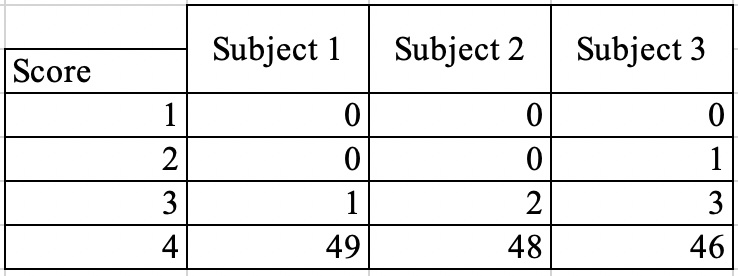
\includegraphics[width=0.8\linewidth]{EffectiveLockChart}
 }
 \caption{\label{EffectiveLockChart} EffectiveLockChart}
 \end{center}
 \end{figure}

Therefore, result of pass due to average engagement without breaking of 95\% of the time when the test force was applied. 

 \begin{figure}[h!]
 \begin{center}
 {
 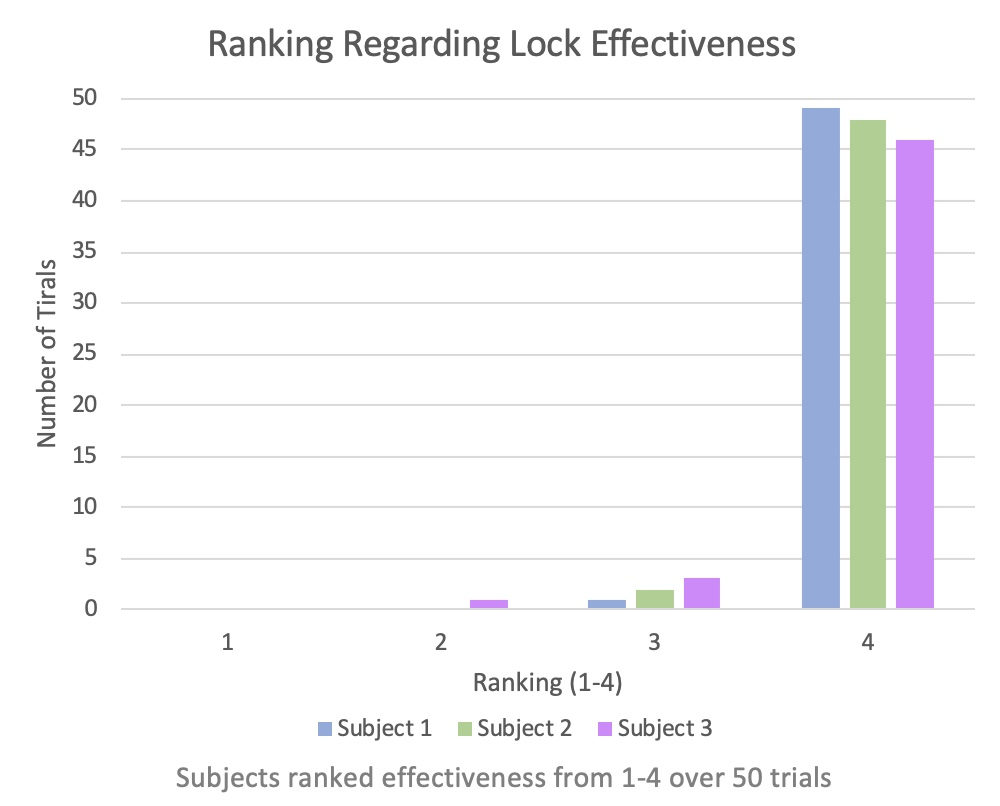
\includegraphics[width=0.65\linewidth]{EffectiveLockGraph}
 }
 \caption{\label{EffectiveLockGraph} EffectiveLockGraph}
 \end{center}
 \end{figure}
 \begin{figure}[h!]
 \begin{center}
 {
 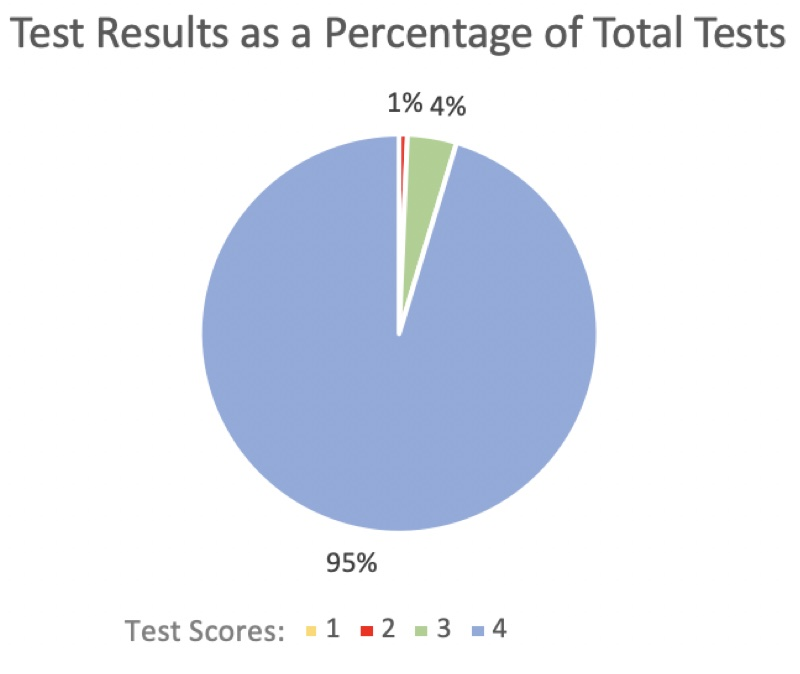
\includegraphics[width=0.65\linewidth]{EffectiveLockGraph2}
 }
 \caption{\label{EffectiveLockGraph2} EffectiveLock Percentage of Tests Resulting in a result of 4}
 \end{center}
 \end{figure}

~\newpage
~\newpage
\item{EffectiveLockSimulation

FR3: Effective Bike Lock: The lock is sturdy and cannot be manually opened by the average human once engaged. }

Expected Results: The CAD simulation meets the 200-400 N threshold. 

Actual Results: Pass -- The CAD simulation is able to meet the 200-400 N threshold. 

\begin{figure}[h!]
\centering
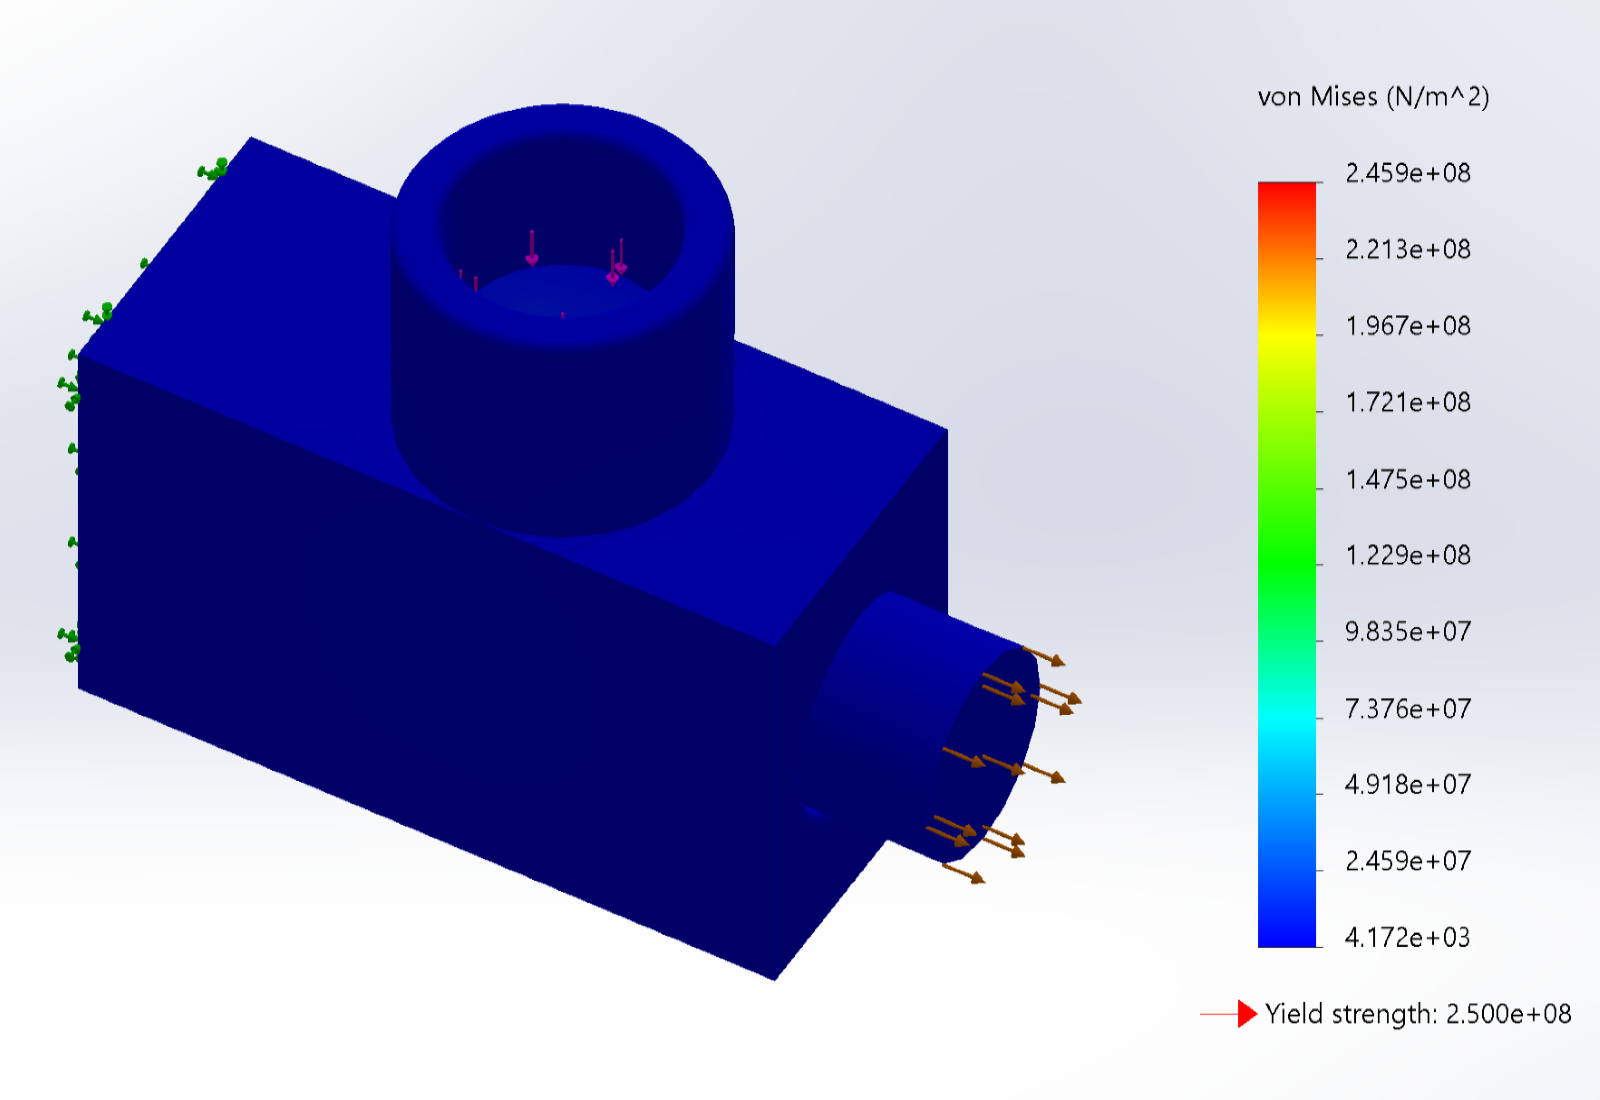
\includegraphics[width=6.7cm]{stress1}
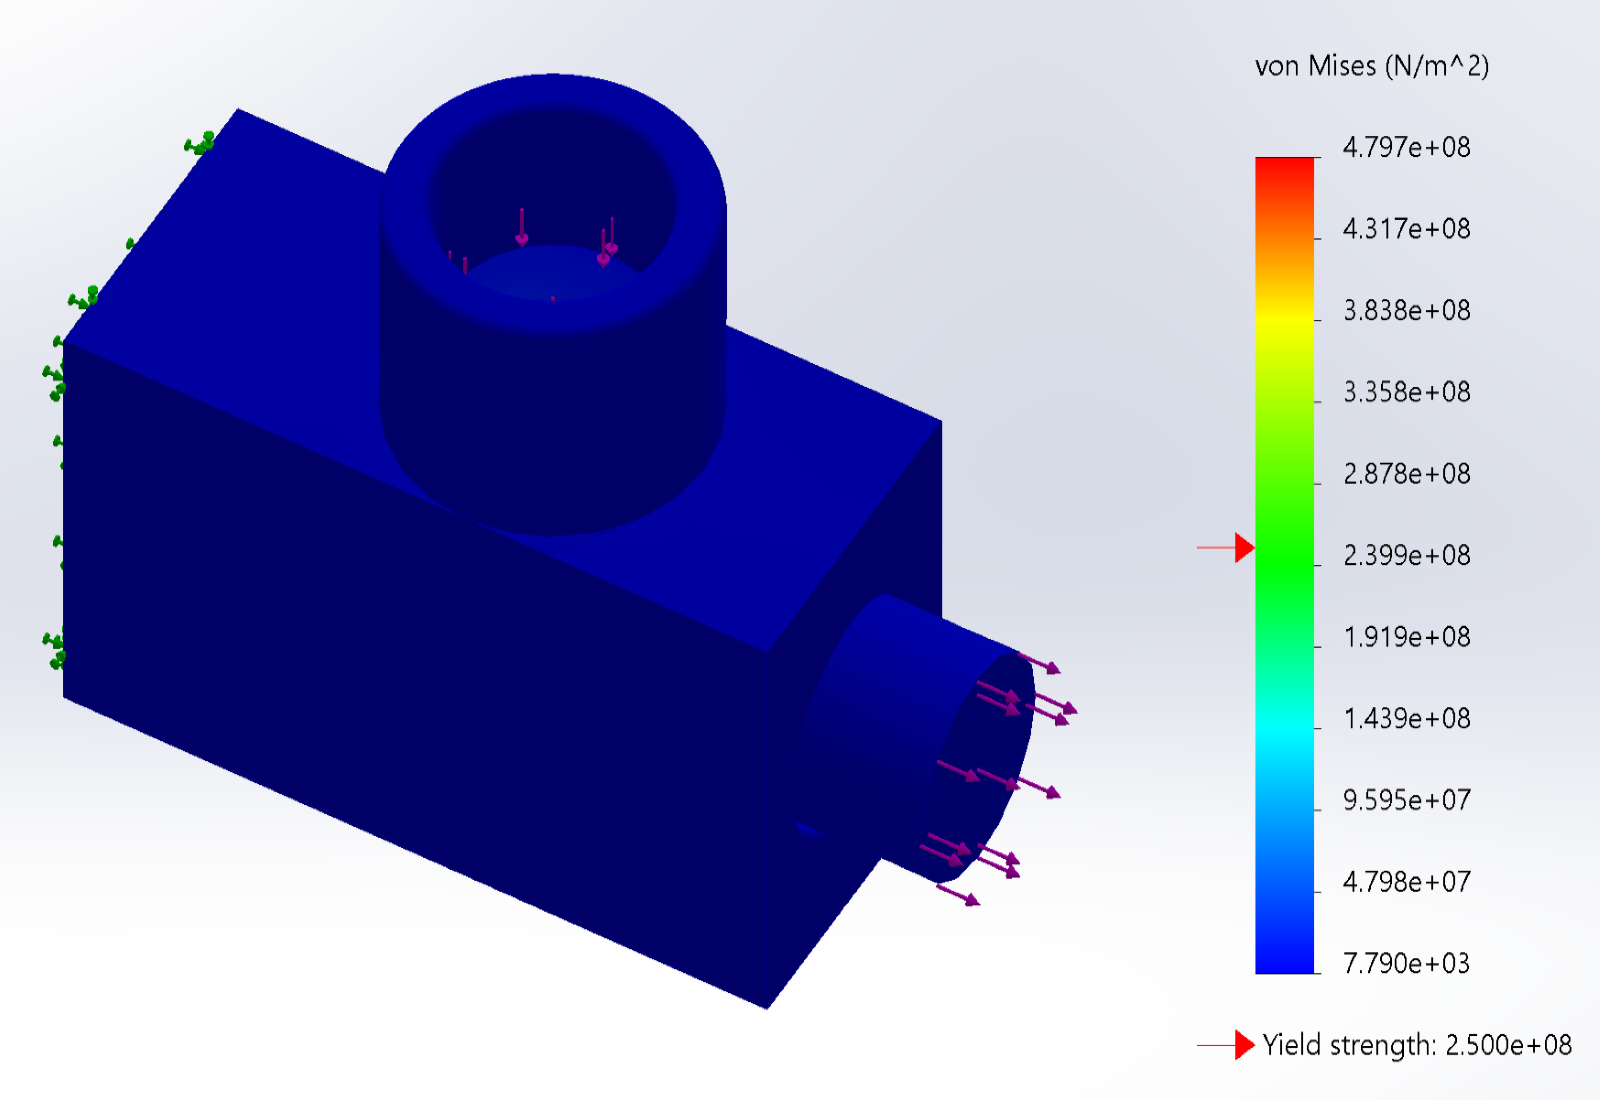
\includegraphics[width=6.7cm]{stress2}
\caption{Stress Results with 200N \& 400N Applied Force}
\end{figure}

\begin{figure}[h!]
\centering
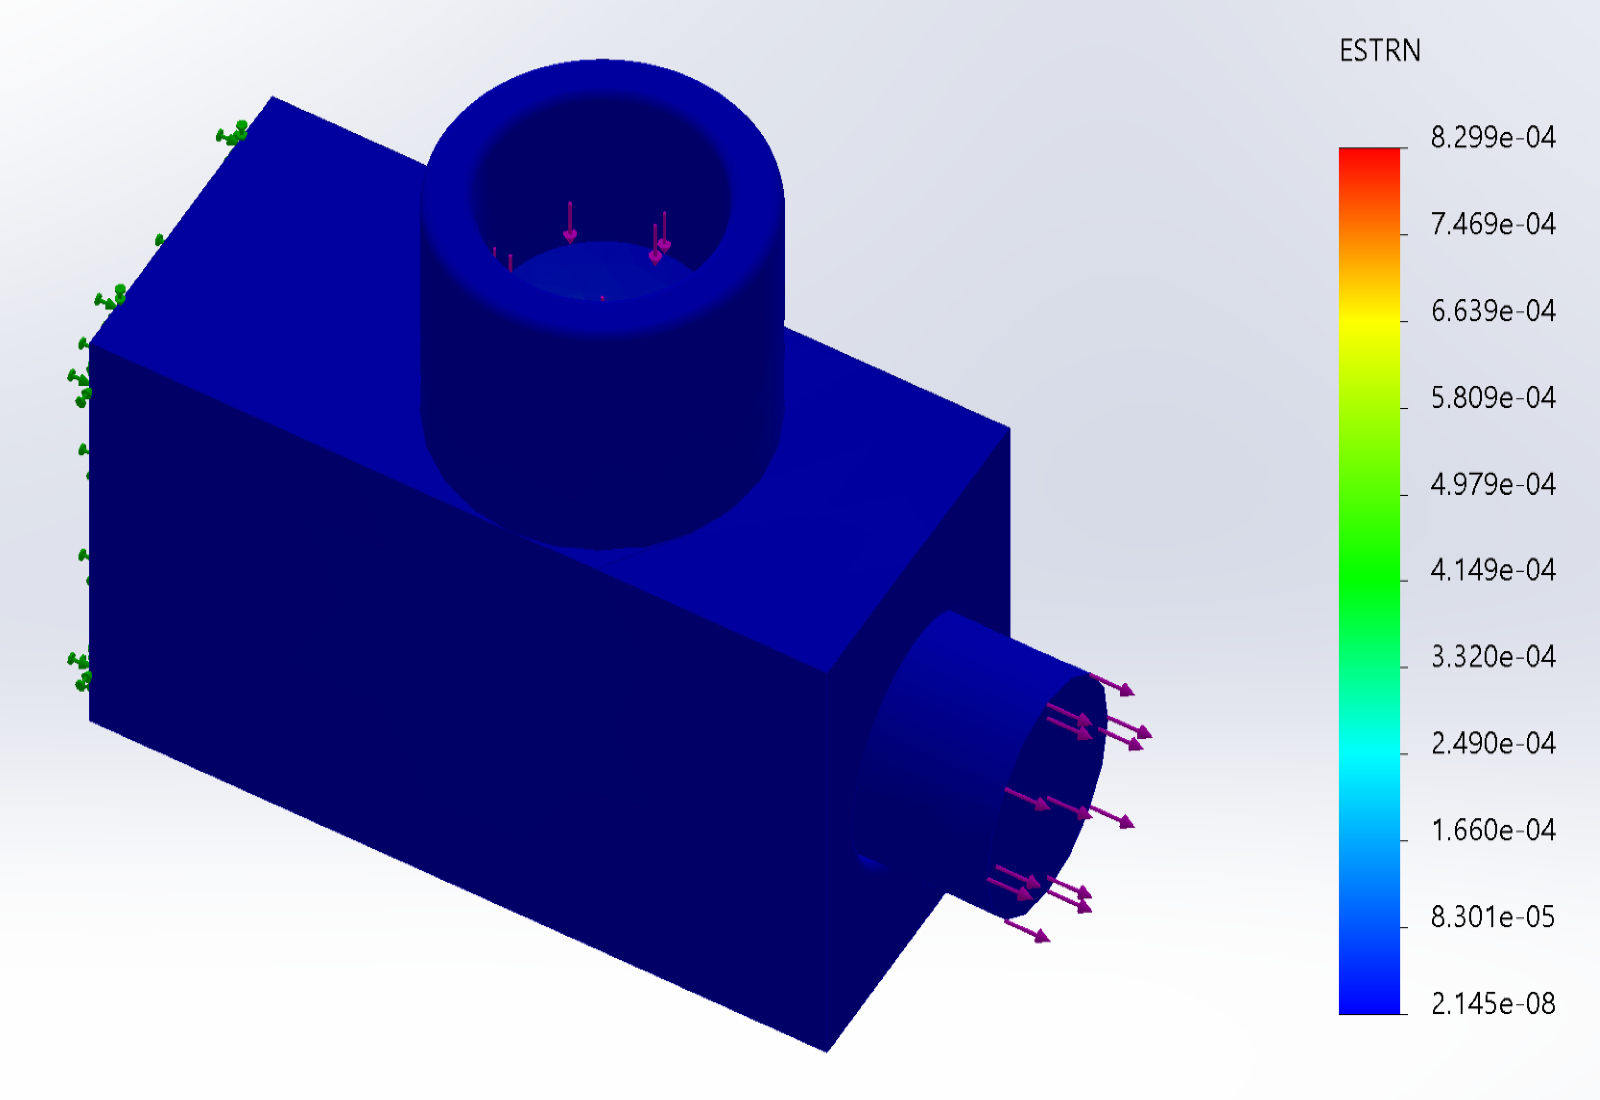
\includegraphics[width=6.7cm]{strain1}
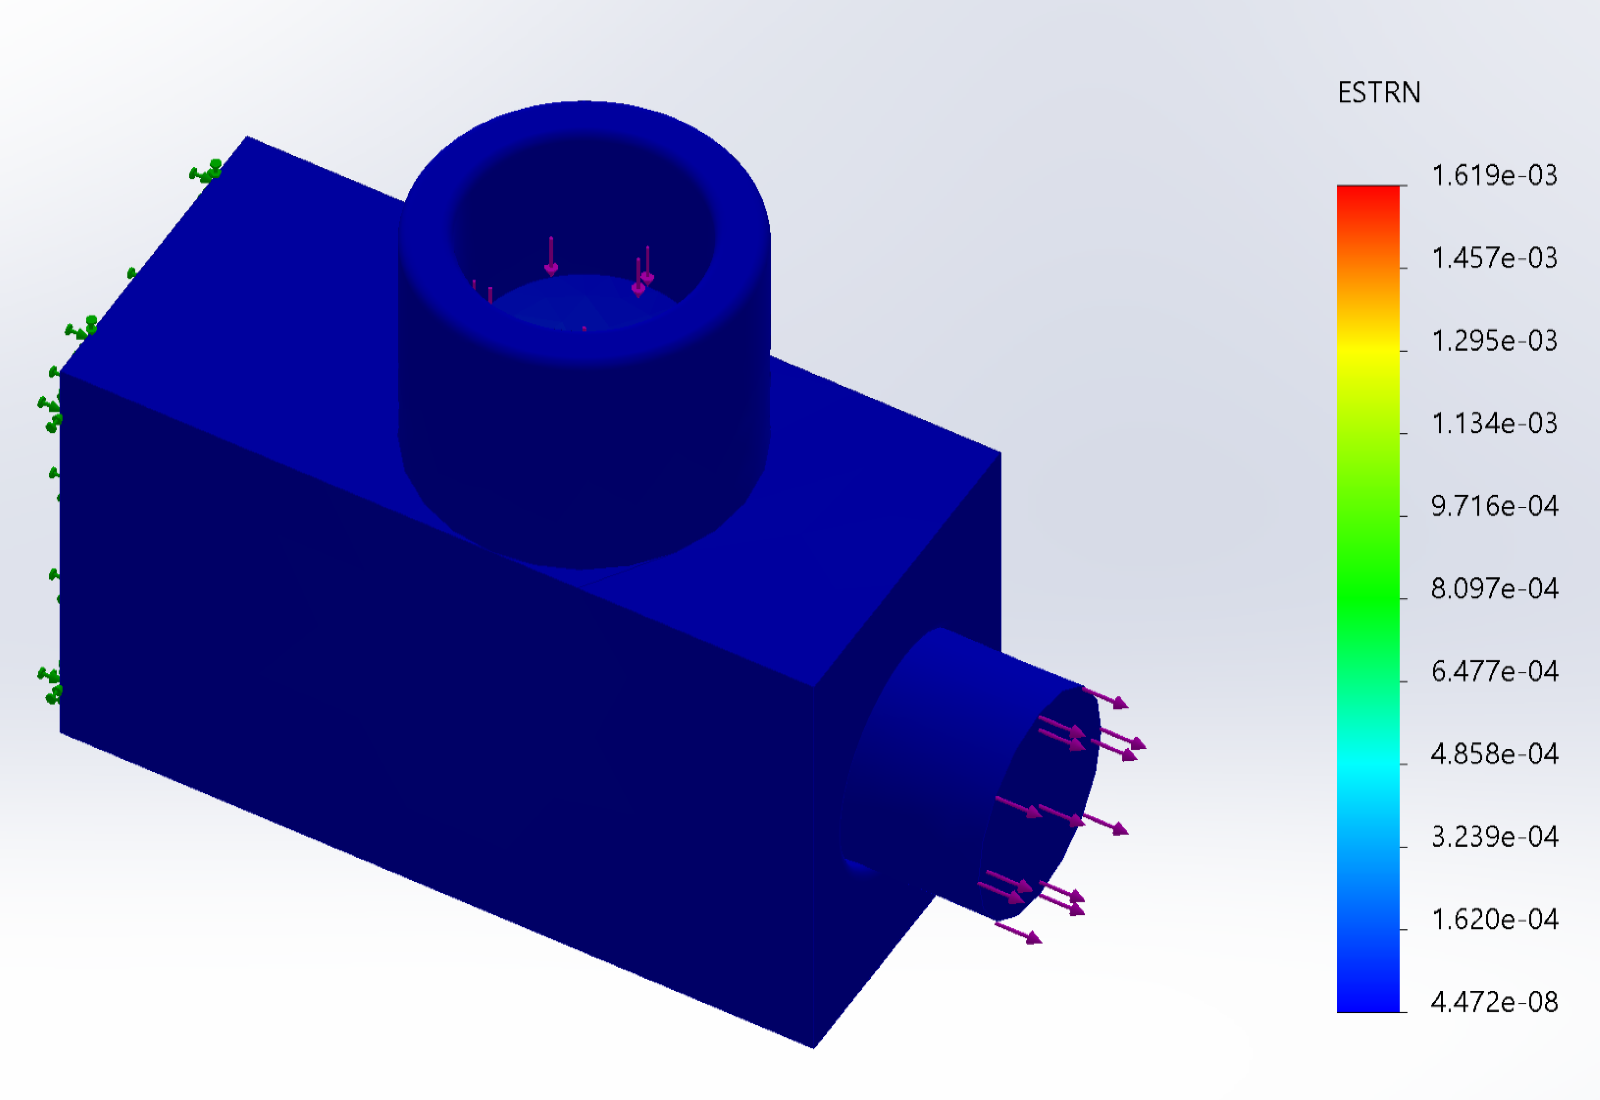
\includegraphics[width=6.7cm]{strain2}
\caption{Stress Results with 200N \& 400N Applied Force}
\end{figure}

\begin{figure}[h!]
\centering
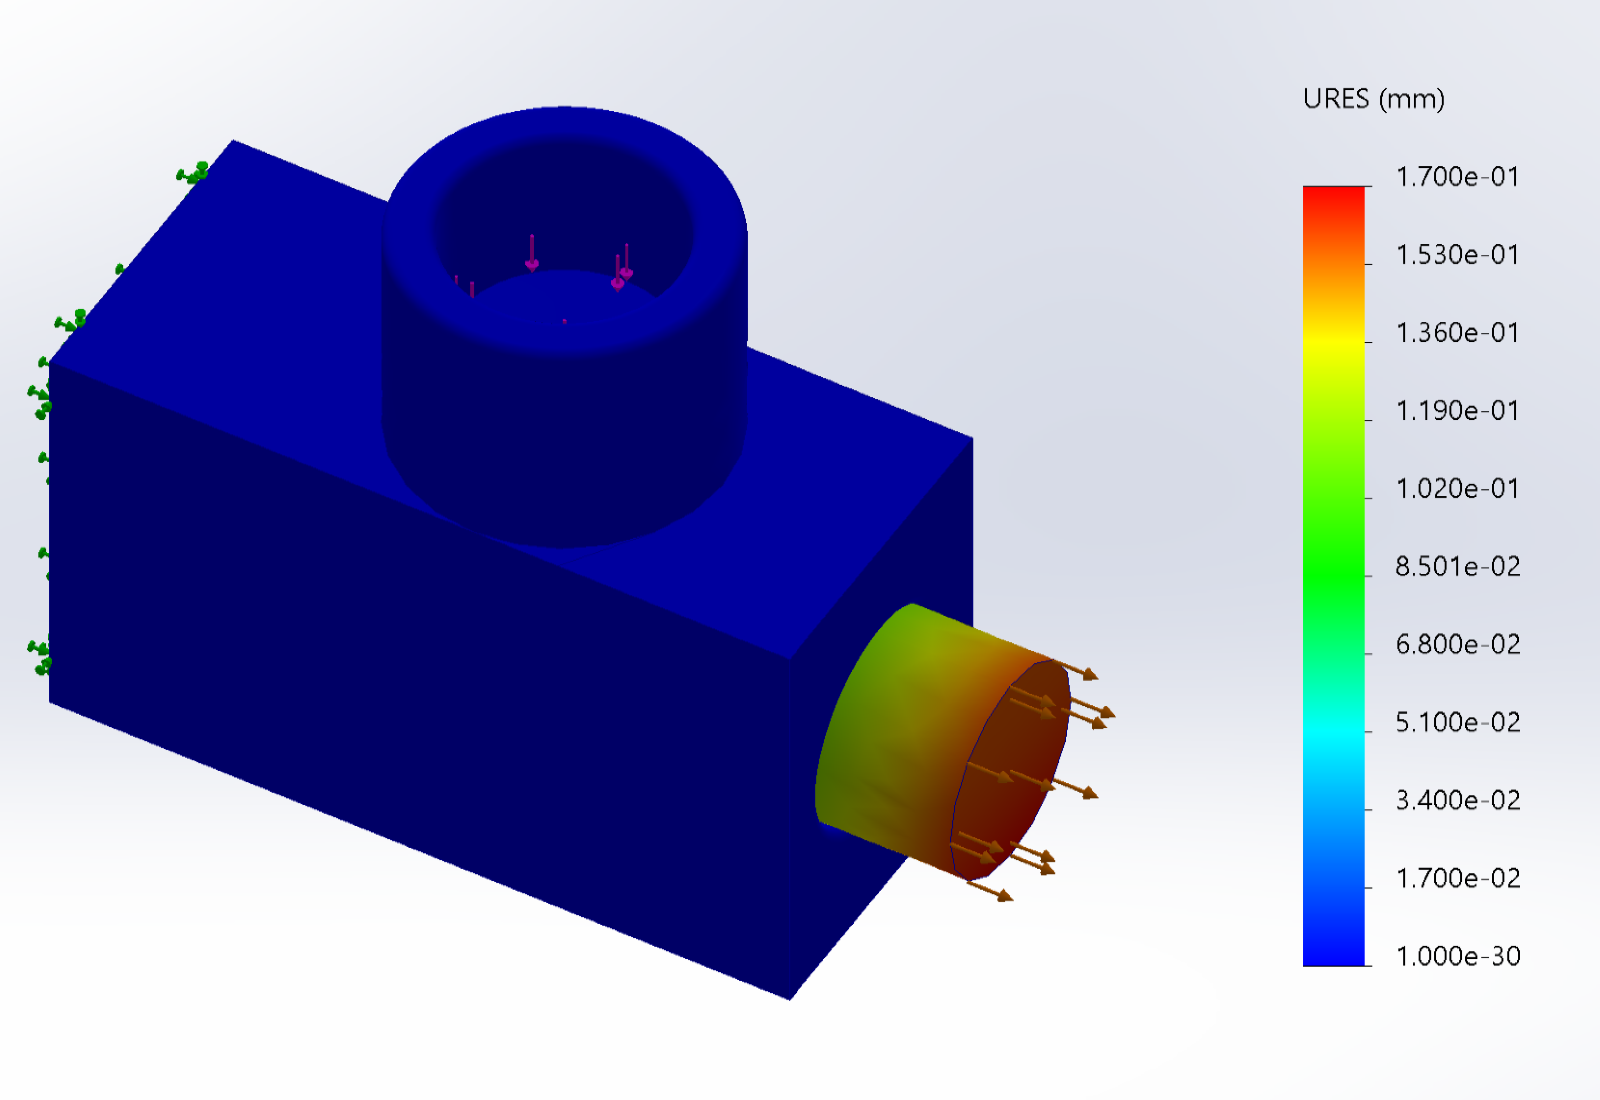
\includegraphics[width=6.7cm]{displacement1}
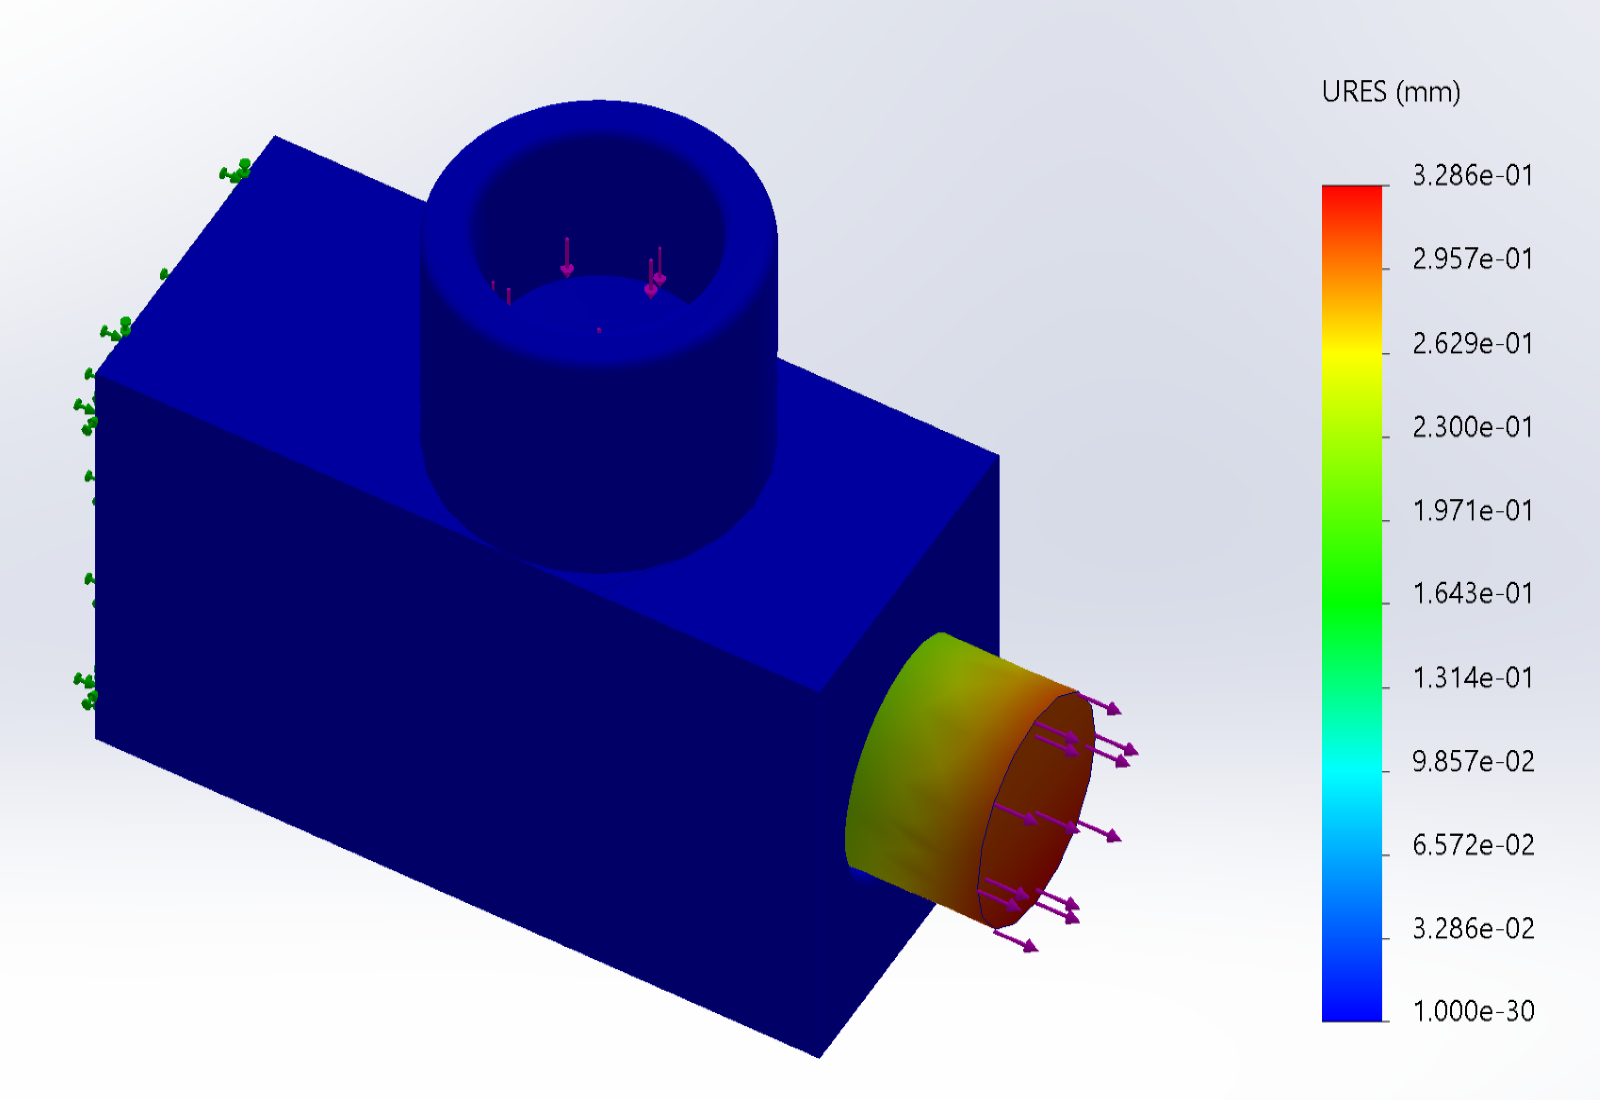
\includegraphics[width=6.7cm]{displacement2}
\caption{Stress Results with 200N \& 400N Applied Force}
\end{figure}

~\newpage


\item{Security

FR4: Lock must only be engaged/disengaged by the intended user(s). }

Expected Results: A Bluetooth developer app is downloaded on an unintended user’s phone. The unintended user will be able to connect to the Arduino but not be able to disengage the lock. 

Actual Results: Pass -- The unintended user was able to connect to the device but not able to unlock the device. 

\end{enumerate}

\subsubsection{Area of Testing: Bike Input Related}

\begin{enumerate}

\item{LockMount

FR5: The lock can be mounted to the bike’s frame. }

Expected Results: A pass/fail per bike tested if the lock is/isn’t able to be mounted onto the bike as intended. A score from 0-the number of bikes tested will be given.  

Actual Results: Three test subjects’ results for the number of bikes where successful lock mounting occurred: 

1 – 3/3 

2 – 3/3 

3 – 3/3 

Therefore, of nine bikes tested, all passed. 

\end{enumerate}

\subsubsection{Area of Testing: Output Related}

\begin{enumerate}

\item{BatteryLevel

FR6: Battery level must be shown on the phone app. }

Expected Results: The user must be able to view the battery level of the lock.

Actual Results: Pass -- The user is able to view the battery level of the lock on the App. It is represented as four levels. 

\item{LocationOnApp

FR7: Location (coordinates) of the bike must be shown on the app as BikePosition.}

Expected Results: The user must be able to view the saved coordinates.

Actual Results: Pass -- The user is able to access and view the saved coordinates of the lock on the App.

\item{PowerOutput

FR8: Battery must output enough power to engage the lock. } \label{PowerOutput}

Expected Results: Circuit connected. Battery is successfully able to meet the threshold voltage of the electromagnet to engage the locking mechanism.  

Actual Results: Pass -- The battery successfully supplied enough voltage to engage the locking mechanism in 5/5 tests. 

Note: During one test where the Arduino was powered on for more than an hour, the battery was supplying the correct voltage, however, the Arduino became defective, (likely due to a current spike), and the locking mechanism was not engaged successfully. Moreover, it was determined that the failed test was due to the Arduino frying, so it was not counted as a failed PowerOutput test. Our learnings from this result are mentioned below in \nameref{Changes Due to Testing}. 

\end{enumerate}

\section{Nonfunctional Requirements Evaluation}

This subset of tests will be used to validate the nonfunctional requirements of our product. Completing these tests will prove various aspects of our product's functionality. These aspects include smartphone app features, the physical design attributes, accuracy, and the usability of the product. Note that each test references, and is directly mapped to, at least one requirement, showing that these test cases robustly cover the defined requirements in the SRS. Note that in this document, only the expected and actual result are listed for each test; for full descriptions (including setup and input) for each test, please refer to the \href{https://github.com/NevoAbigail/Capstone/blob/main/docs/VnVPlan/VnVPlan.pdf}{VnV Plan}.

\subsubsection{Area of Testing: Smart Phone}

\begin{enumerate}

\item{LimitedInstructions

NFR1: Can reasonably be used without requiring an instruction manual. }

Expected Results: The lock is successfully engaged and disengaged, and the bike is securely locked by all test users.

Actual Results: Three test users were able to successfully engage and disengage the lock without instruction. The bikes were then tested to be securely locked by attempting to unlock them manually, (disengage the locking mechanism), with an average human's arm strength. 

\item{AppStorage

NFR2: App storage under 50 megabytes. A small mobile app should not take up significant space on the user’s phone.  }

Expected Results: App storage is less than 50 MB. 

Actual Results: Pass -- App storage does not exceed 50 MB. 

\end{enumerate}

\subsubsection{Area of Testing: Physical Lock}
\begin{enumerate}

\item{VisualAppeal

NFR3: The design must be visually appealing.}

Expected Results: Survey users on their opinions of the visual appeal of the device; see \nameref{User Testing}, question 6. A majority of surveyed users should deem the visual appeal satisfactory--a rating of 5 or above.

Actual Results: The majority of surveyed users deemed the visual appeal of the SmartLock satisfactory (rating of 5) or above expectations. 

 \begin{figure}[h!]
 \begin{center}
 {
 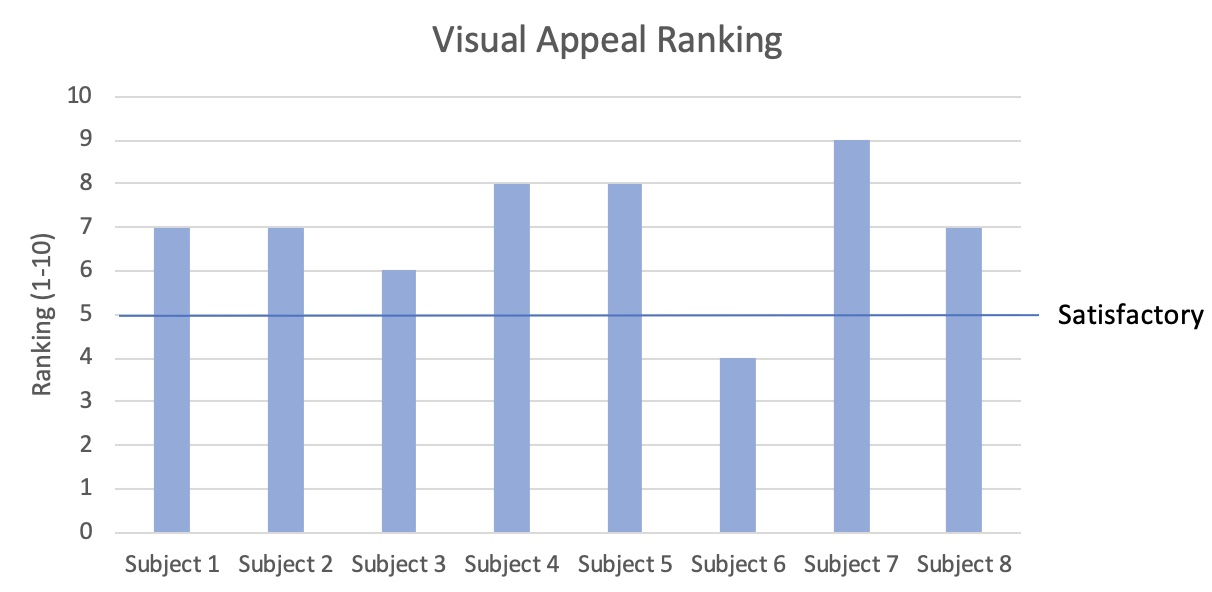
\includegraphics[width=0.65\linewidth]{VisualAppealRanking}
 }
 \caption{\label{VisualAppealRanking} Visual Appeal Ranking}
 \end{center}
 \end{figure}

~\newpage
\item{NormalBikeFunction

NFR4: The lock must not impede normal bike functions. }

Expected Results: The SmartLock does not impede normal bike functionality and operation. 

Actual Results: Pass -- The SmartLock does not impede normal bike functionality and operation. 

\item{Safety

NFR5: The design must not inflict harm to the user in any way, such as clamping down on a finger, or moving at a force or speed that could cause injury. }

Expected Results: The design must not inflict harm to the user in any way, such as clamping down on a finger, or moving at a force or speed that could cause injury. 

Actual Results: Pass -- User is not harmed or pinched when SmartLock is in use. 

\end{enumerate}

\subsubsection{Area of Testing: Accuracy}

\begin{enumerate}

\item{BatteryAccuracy

NFR6: Battery level must be calculated accurately within 25\% since it uses four battery levels.}

Expected Results: The number of lock engages possible with 1\% battery matches our specification for the number of lock engages possible with 100\% battery (multiply the measured \# of lock engages possible with 1\% battery by 100), within 25\% accuracy.

Actual Results: The number of lock engages possible with 1\% and 100\% battery level was manually tested and compared to the calculated number. It was within the required 25\% accuracy. 

\end{enumerate}

\subsubsection{Area of Testing: Usability}

\begin{enumerate}

\item{QuickLock

NFR7: The SmartLock must be quicker to use than a typical keyed or combination bike lock.  }

Expected Results: The SmartLock must be quicker to use than both a  sample keyed and combination lock. One test user will attempt three times each to lock and unlock typical keyed and combination as well as the SmartLock. All tests must be faster for the SmartLock.

Actual Results:


\begin{figure}[h!]
 \begin{center}
 {
 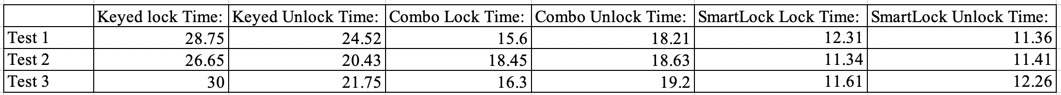
\includegraphics[width=1\linewidth]{QuickLockChart}
 }
 \caption{\label{QuickLockChart} QuickLockChart}
 \end{center}
 \end{figure}
 \begin{figure}[h!]
 \begin{center}
 {
 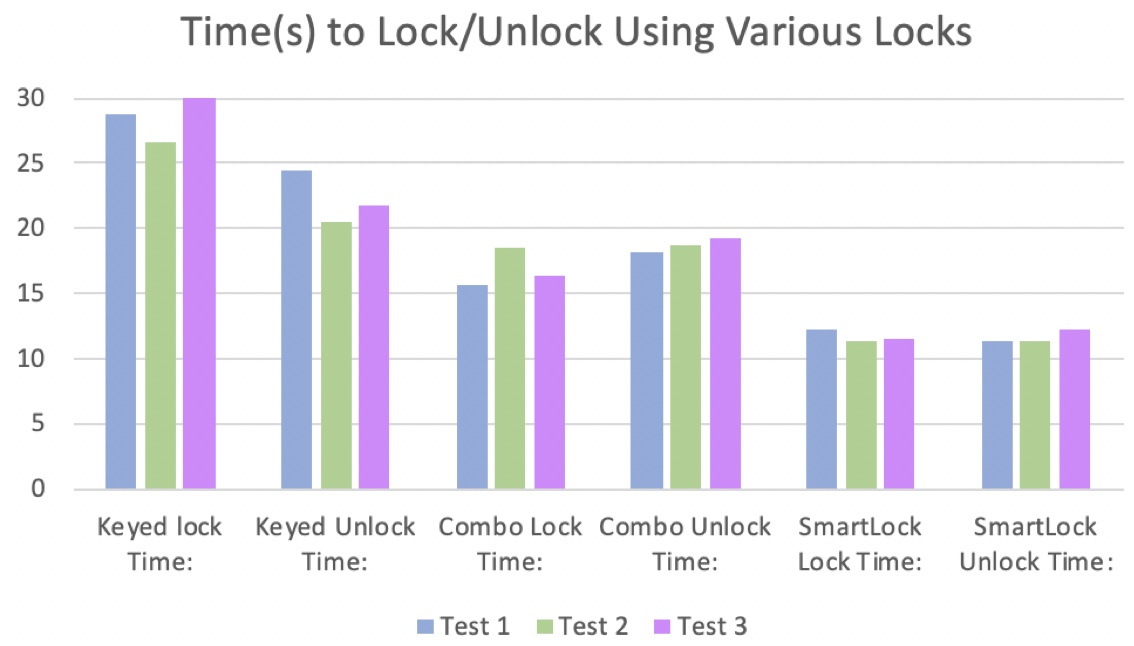
\includegraphics[width=1\linewidth]{QuickLockGraph}
 }
 \caption{\label{QuickLockGraph} QuickLockGraph}
 \end{center}
 \end{figure}

~\newpage
\item{UseForce

NFR8: Opening and closing lock must require similar force to a typical keyed/combo.  }

Expected Results: The amount of force required to open and close the lock frame is comparable to that of a typical keyed or combination lock. Test users score the force required out of 5 where 5 is the maximum amount of force they can physically provide and 1 is the minimum amount of force they can physically provide. The SmartLock should not vary more than 1 score unit from the most different score in each test. 

Actual Results: Three tests subjects’ results for the amount of force required to open and close the lock frame for the SmartLock, a typical keyed lock and a combination lock respectively out of 5: 

1- 2, 1, 2 

2- 3, 3, 3 

3- 1, 1, 2 

Therefore, the SmartLock did not vary more than one score unit from the most different score in each test. 

\item{BatteryLife

NFR9: Battery must last for greater than 1 month and/or 60 rides before needing to be replaced or charged.  }

Expected Results: The battery lasts for longer than 1 month and/or 60 rides before needing to be replaced or charged. 

Actual Results: Pass -- The battery lasted longer than 1 month before needing to be replaced or charged. 

\item{ComponentAccessibility

NFR10: Batteries and other internal components must be accessible to replace and/or chargeable. }

Expected Results: The battery can be replaced, and internal components can be accessed, as intended.

Actual Results: Pass -- Three test users were able to access and replace the battery and all other internal components.  

\item{NoSpecialTools

NFR11: The lock must be easily mounted on the bike frame. It does not require special tools, (i.e., those not found in a typical toolbox, such as power tools), to be installed and does not take more than twenty minutes to install. }

Expected Results: The lock is easily mounted on the bike frame. It does not require special tools, (i.e., those not found in a typical toolbox, such as power tools), to be installed and does not take more than twenty minutes to install.  

Actual Results: Three test subjects’ results for three individual tests for the time to mount the lock on their bike frame without the use of special tools.  

1 -- 6, 5, 4 min 

2 -- 7, 7, 4 min 

3 – 5, 3, 3 min 

Therefore, all tests were successful and completed within twenty minutes. 

\item{BikeVersatility

NFR12: The lock can be used for many different models of mountain, city, and road bikes.  }

Expected Results: The SmartLock can be mounted on three different categories of bikes (road, hybrid and mountain) successfully by each test user.  

Actual Results: Three test subjects’ results for the number of bikes where successful lock mounting occurred: 

1 – 3/3 

2 – 3/3 

3 – 3/3 

Therefore, of nine bikes from three different types of bikes (road, hybrid and mountain) tested, all passed. 

\item{AppOS

NFR17: The App should run on iOS and Android.  }

Expected Results: App operates on iOS and Android. 

Actual Results: Pass -- App operates successfully on iOS and Android as expected. 

\end{enumerate}

\section{Unit Testing}

Please refer to Section 5: Unit Testing of the \href{https://github.com/NevoAbigail/Capstone/blob/main/docs/VnVPlan/VnVPlan.pdf}{Verification and Validation Plan} for details of each unit test, including setup, input, and expected result. A summary table of the results of this testing is provided below. A passing result is one where the actual result matches the expected result. 

\captionof{table}{Unit Testing Results Table}
\begin{center}

\begin{tabular}{|c|c|}
  \hline
  \textbf{\href{https://github.com/NevoAbigail/Capstone/blob/main/docs/VnVPlan/VnVPlan.pdf}{Unit Test}} & \textbf{Result} \\
  \hline
  Locking Mechanism & PASS\\
  \hline
  Arduino Bluetooth Connection & PASS\\
  \hline
  Arduino Disengage Signal Output & PASS\\
  \hline
  Arduino Incorrect Password Signal Output & PASS \\
  \hline
  Circuit Transistor Test & PASS \\
  \hline
  Circuit Solenoid Test & PASS \\
  \hline
  Full Circuit Test & PASS \\
  \hline
  
\end{tabular}
\end{center}

\section{User Testing} \label{User Testing}

Eight users were asked to try the SmartLock, and were asked several questions about their experience. These questions can be found in the \href{https://github.com/NevoAbigail/Capstone/blob/main/docs/VnVPlan/VnVPlan.pdf}{VnV Plan}, and are also reiterated here, with the common answers we received.

\begin{enumerate}
    \item How long does it take you to open the lock? Is a 5-second window too short? Too long?

    5 seconds was found to be just slightly too short of an unlock window. It was found that 10 seconds was enough time to pull the pin out of the body of the lock. This change will be implemented. 
    
    \item Is the app intuitive to use? Would you change any features or any part of the app design?

    Many users commented on not being able to get directions based on the location they geotagged. 
    
    \item How did you like the whole product use experience? Is the locking/unlocking process smooth, convenient, and efficient?

    Especially due to the current cold weather, users enjoyed not needing to fiddle with a key or combination lock, and just being able to press a button to unlock their bike. 
    
    \item Was any aspect of using the product confusing?

    Again, users commented on the listing of all Bluetooth devices as being confusing. Users also mentioned that it was not clear that the lock would only be disengaged for a limited period of time after pressing "Unlock". This concept must be clarified either within the app, or in a separate instruction manual. Further, users commented on the order (from the top to bottom) of the buttons on the app, and suggested a reordering of some buttons might make it easier to use.
    
    \item Would you be comfortable using this product to lock your bike? What would make you feel more secure?

    Due to all of the internal components currently being not secured properly, and the solenoid being exposed to the outside, most users said they were not comfortable using the SmartLock. In order to make the lock more secure, the housing could be redesigned to hold all of the components internally. 
    
    \item Rate this device's visual appeal on a scale of 1-10, with 10 being the most visually appealing, and 1 being the least visually appealing.
    
    Most users were satisfied with the visual appeal of the App and the SmartLock's physical features. The results of this survey can be found in the \nameref{VisualAppealRanking} graph.
    
\end{enumerate}

\section{Changes Due to Testing} \label{Changes Due to Testing}

%\wss{This section should highlight how feedback from the users and from 
%the supervisor (when one exists) shaped the final product.  In particular 
%the feedback from the Rev 0 demo to the supervisor (or to potential users) 
%should be highlighted.}

Changes due to Requirement Testing are summarized below:
\begin{enumerate}
    \item Add a diode across the electromagnet in order to protect the transistor from the inductive voltage spike which occurs as the solenoid de-energizes. As deemed necessary from the \hyperref[PowerOutput]{Power Output Test}
    \item Add a moderately-sized gate resistor between the gate of the MOSFET and the Arduino to protect the Arduino from current spikes. As deemed necessary from the \hyperref[PowerOutput]{Power Output Test}
\end{enumerate}

Changes due to \nameref{User Testing} are summarized below:

\begin{enumerate}
    \item Change the lock disengaged window (how long the lock is disengaged after pressing "Unlock") to 10 seconds from 5 seconds, as suggested by users' answer to the question "How long does it take you to open the lock? Is a 5-second window too short? Too long?"
    \item Display coordinates of geotagged/pinned location on app. This way, users can then copy these coordinates and paste them into a map app of their choosing to get directions. This change was prompted by users' answers to the question "Is the app intuitive to use? Would you change any features or any part of the app design?"
    \item Redesign the App UI to make it more user-friendly and intuitive, as prompted by users' answers to the question, "Was any aspect of using the product confusing?"
 
\end{enumerate}

\section{Automated Testing} \label{Automated Testing}

As mentioned in the \href{https://github.com/NevoAbigail/Capstone/blob/main/docs/VnVPlan/VnVPlan.pdf}{VnV Plan}, we used a few tools for automated testing and verifying coding standards.

\begin{enumerate}
    \item CodeFactor

    After importing our project repository into CodeFactor, we recieved a grade A for code quality.

    \begin{figure}[h!]
    \centering
    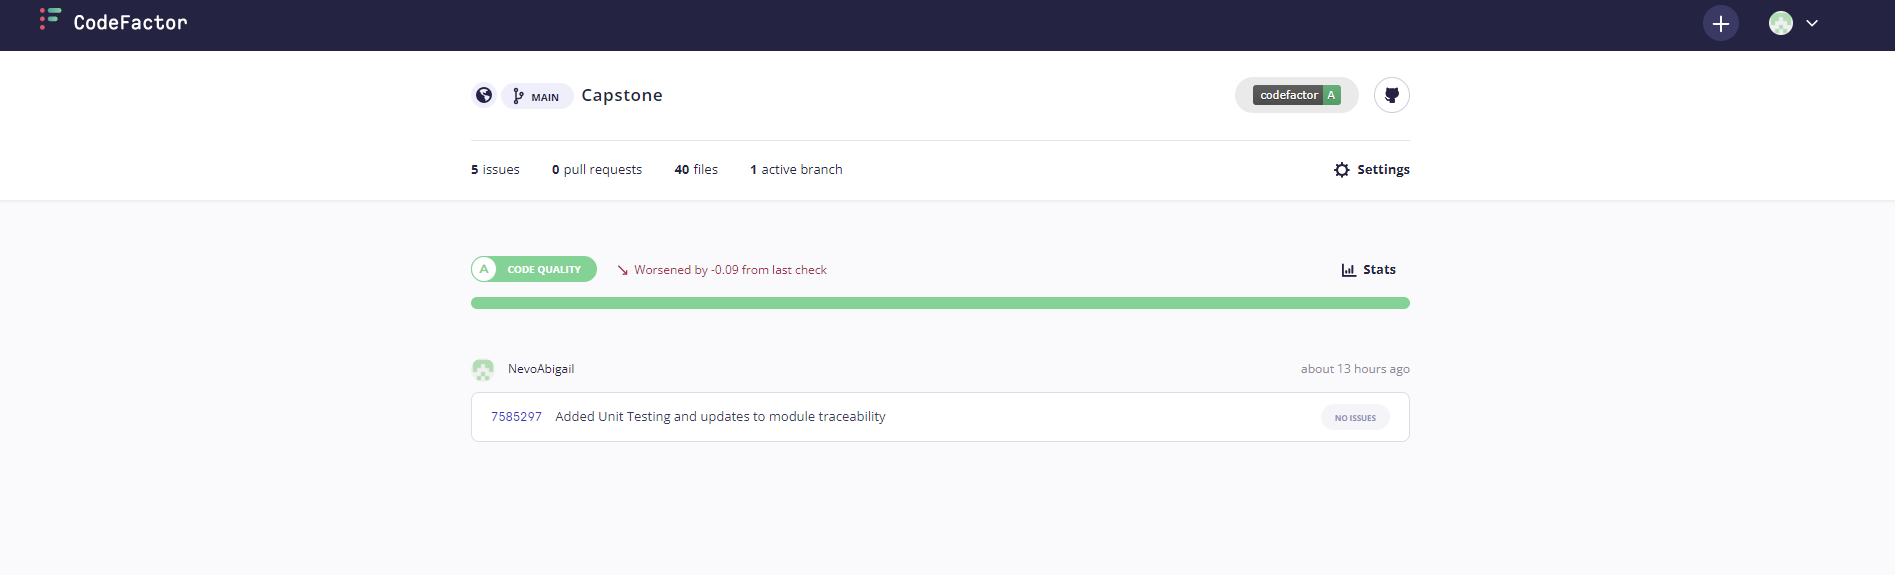
\includegraphics[width=15cm]{CodeFactor}
    \caption{CodeFactor Results}
    \end{figure}

\end{enumerate}
		
\section{Trace to Requirements}

\begin{minipage}{\textwidth}
\footnotesize
\captionof{table}{Requirements Traceability Table}
\renewcommand*{\arraystretch}{1.5}
\begin{tabular}{| p{0.3\textwidth} | p{0.4\textwidth} | p{0.4\textwidth} |}
 \hline
 Test Case & \href{https://github.com/NevoAbigail/Capstone/blob/main/docs/SRS/SRS.pdf}{Functional Requirement(s)} & \href{https://github.com/NevoAbigail/Capstone/blob/main/docs/SRS/SRS.pdf}{Non-Functional Requirement(s)} \\ 
 \hline
 DisengageLock & FR1 &  \\ 
  \hline
 LockLocation & FR2 &  \\ 
  \hline
 EffectiveLock, EffectiveLockSimulation & FR3 &  \\ 
  \hline
 Security & FR4 &  \\ 
  \hline
 LockMount & FR5 &  \\ 
  \hline
 BatteryLevel & FR6 &  \\ 
  \hline
 LocationOnApp & FR7 &  \\ 
  \hline
 PowerOutput & FR8 &  \\ 
  \hline
 LimitedInstructions & & NFR1 \\
 \hline
  AppStorage & & NFR2 \\
 \hline
  VisualAppeal & & NFR3 \\
 \hline
  NormalBikeFunction & & NFR4 \\
 \hline
  Safety & & NFR5 \\
 \hline
  BatteryAccuracy & & NFR6 \\
 \hline
  QuickLock & & NFR7 \\
 \hline
 UseForce & & NFR8 \\
 \hline
 BatteryLike & & NFR9 \\
 \hline
  ComponentAccessibility & & NFR10 \\
 \hline
  NoSpecialTools & & NFR11 \\
 \hline
  BikeVersatility & & NFR12 \\
 \hline
  AppOS & & NFR17 \\
 \hline
 \end{tabular}
\end{minipage}\\

Note: NFR 13-16 and 18 were deemed out of scope on the SRS, and thus are not present in this Verification and Validation Plan. 
		
\section{Trace to Modules}	

\begin{minipage}{\textwidth}
\footnotesize
\captionof{table}{Modules Traceability Table}
\renewcommand*{\arraystretch}{1.5}
\begin{tabular}{| p{0.5\textwidth} | p{0.5\textwidth} |}
 \hline
 Test Case & \href{https://github.com/NevoAbigail/Capstone/blob/main/docs/Design/SoftArchitecture/MG.pdf}{Module(s)}  \\ 
 \hline
 DisengageLock & Hardware Disengage \\ 
  \hline
 LockLocation & Location \\ 
  \hline
 EffectiveLock, EffectiveLockSimulation & Solenoid Actuation, Locking Mechanism  \\ 
  \hline
 Security & Hardware Disengage\\ 
  \hline
 LockMount & Lock Frame \\ 
  \hline
 BatteryLevel & Battery, Battery Status \\ 
  \hline
 LocationOnApp & Location \\ 
  \hline
 PowerOutput & Battery, Solenoid Actuation \\ 
  \hline
 LimitedInstructions & None \\
 \hline
  AppStorage & Location, Battery Status, Mobile App Bluetooth Communication and User Disengage \\
 \hline
  VisualAppeal & Lock Frame,  Mobile App Bluetooth Communication and User Disengage, Battery Status, Location \\
 \hline
  NormalBikeFunction & Lock Frame \\
 \hline
  Safety & Lock Frame, Locking Mechanism \\
 \hline
  BatteryAccuracy & Battery, Battery Status \\
 \hline
  QuickLock & Locking Mechanism,  Mobile App Bluetooth Communication and User Disengage, Solenoid Actuation \\
 \hline
 UseForce & Locking Mechanism\\
 \hline
 BatteryLife &  Mobile App Bluetooth Communication and User Disengage, Location, Battery Status, Battery \\
 \hline
  ComponentAccessibility & None \\
 \hline
  NoSpecialTools & Lock Frame \\
 \hline
  BikeVersatility & Lock Frame \\
 \hline
  AppOS &  Mobile App Bluetooth Communication and User Disengage, Location, Battery Status \\
 \hline
 \end{tabular}
\end{minipage}\\

Note: NFR 13-16 and 18 were deemed out of scope on the SRS, and thus are not present in this Verification and Validation Plan. 


\bibliographystyle{plainnat}
\bibliography{../../refs/References}

\newpage{}
\section{Appendix}
\subsection{Reflection}

The information in this section will be used to evaluate the team members on the
graduate attribute of Reflection.  Please answer the following question:

\begin{enumerate}
  \item In what ways was the Verification and Validation (VnV) Plan different
  from the activities that were actually conducted for VnV?  If there were
  differences, what changes required the modification in the plan?  Why did
  these changes occur?  Would you be able to anticipate these changes in future
  projects?  If there weren't any differences, how was your team able to clearly
  predict a feasible amount of effort and the right tasks needed to build the
  evidence that demonstrates the required quality?  (It is expected that most
  teams will have had to deviate from their original VnV Plan.)
  
  The VnVPlan was different than the actual VnV because several of the tests were initially hoped to be broader, however the group decided to utilize our time more effectively by making the tests more concise but still useful. In other words--we had to limit our scope. For example, instead of conducting surveys over 50 or 100 people, we limited our user testing to less than 10. We overestimated how much time we would have to complete testing, and were not thinking about completing the tests realistically. 

Some of our tests were also not extremely founded or based in reality. For example, we said in the VnV Plan we would test the durability of the product by dropping/kicking/hitting it, but in reality, we obviously don't want to accidentally break our project in doing so. Instead, we used a CAD simulation to show how strong the SmartLock is, and didn't have to physically try to break the product. 

In future projects, when creating the VnV plan, it would be helpful to realistically think about what your team can accomplish in your time frame, and with the current resources you have access to. If you say, "apply a force of XX N", take the time to think through how you will apply this force, how you will know if the correct amount of force is being applied, and also why this is the specific amount of force necessary to test. Further, think about the consequences if the test fails--if you try to test the limits of your product and it breaks, what happens then? Is there an alternative simulation/test that can be completed instead?
\end{enumerate}

\end{document}